%  !TeX  root  =  user_guide.tex

\section{SQL Anywhere}\label{sec:sqlanywhere}

% when the revision of a section has been finalized,
% comment out the following line:
% \updatedisclaimer

SQL Anywhere проприетарная реляционная система управления базами данных
(РСУБД), разрабатываемая компанией Sybase. В SQL Anywhere 12 появилась
поддержка пространственных данных, включая поддержку стандартов OGC и
SQLMM, инструментарий для импорта shape-файлов и встроенные функции для
экспорта в форматы KML, GML и SVG.

Модуль \toolbtntwo{sqlanywhere}{SQL Anywhere} позволяет подключаться к
просторанственным базам данных SQL Anywhere. Диалоговое окно \dialog{Добавить слой SQL Anywhere}
повторяет функционал диалоговых окон провайдеров PostGIS и SpatiaLite.

\begin{figure}[ht]
   \centering
   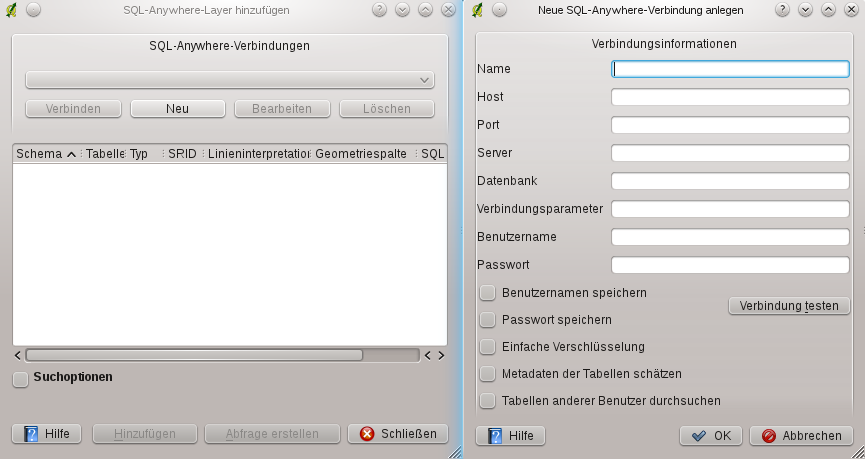
\includegraphics[clip=true, width=14cm]{sql_anywhere}
   \caption{Окно модуля SQL Anywhere \nixcaption}
   \label{fig:sqlanywhere}
\end{figure}

%% FIXME Needs an example, but the database is proprietary

\FloatBarrier
